\documentclass[11pt]{article}
%Gummi|065|=)
\usepackage{graphicx}
\usepackage[utf8]{inputenc}
\usepackage[top=2cm, bottom=2cm, left=2cm, right=2cm]{geometry}
\usepackage{fancyhdr}
\usepackage{lastpage}
\usepackage{verbatim}
\usepackage{graphicx}
\usepackage{float}
\usepackage{wrapfig}
\usepackage{amssymb,amsmath}

\title{\textbf{Rapport - Modélisation et Simulation de l'Excitation Cardiaque}}
\author{Hadrien Titeux \& Thomas Ghesquiere}

\newcounter{question_num}
\setcounter{question_num}{1}


\date{}
\begin{document}

\maketitle

\section{Modélisation et discrétisation}
	\paragraph{Question \arabic{question_num} \\}
	La fonction $ euler1 $ permet de caluler $ u_{n} $ au temps t suivant en utilisant la méthode d'Euler. Cette fonction fonctionne aussi pour des vecteurs.
	
	\stepcounter{question_num}
	\paragraph{Question \arabic{question_num} \\}
	Pour vérifier la fonction euler1, nous allons la tester avec le systéme suivant :
	\[
	\left\{
	\begin {array}{r c l}
	\frac{du(t)}{dt} =& -0.1 t \ u(t) & \forall t < 50 \\
	u_{0}=& 1
	\end {array}
	\right.
	\]
	La solution de ce systéme est :
	\[
	\forall t < 50, \ u(t)=e^{0.05 \ t^2}
	\]
	Nous pouvons donc comparer la courbe réelle à celle obtenue avec la méthodes d'euler et ainsi vérifier la fonction $euler1$.
	\begin{figure}[H]
	\begin{center}
		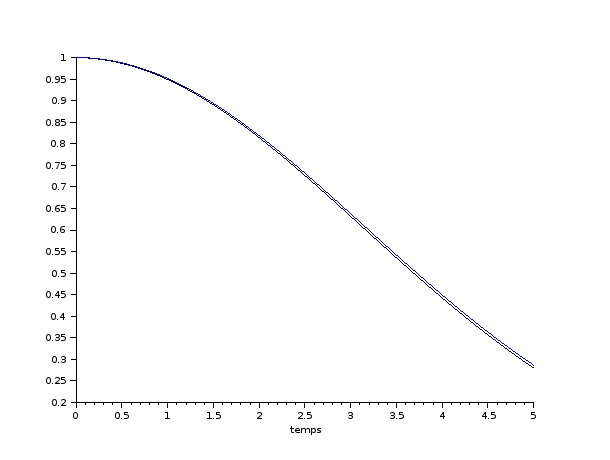
\includegraphics[width=8 cm]{question2.jpeg}
		\caption{ Graphique de comparaison}
	\end{center}
	\end{figure}
	
	Les deux courbes obtenues se superposent parfaitement. Il suffit de diminier le pas $dt$ pour ne plus pouvoir les distinguer. La fonction $euler1$ permet donc bien de résoudre les systémes du même type que celui-ci.
	
	\stepcounter{question_num}
	\paragraph{Question \arabic{question_num} \\}
 	titeux	

	\stepcounter{question_num}
	\paragraph{Question \arabic{question_num} \\}
	Nous allons donc résoudre le modéle cellulaire proposé avec la fonction $euler1$. Voila les courbes des solutions approchées :
	\begin{figure}[H]
	\begin{center}
		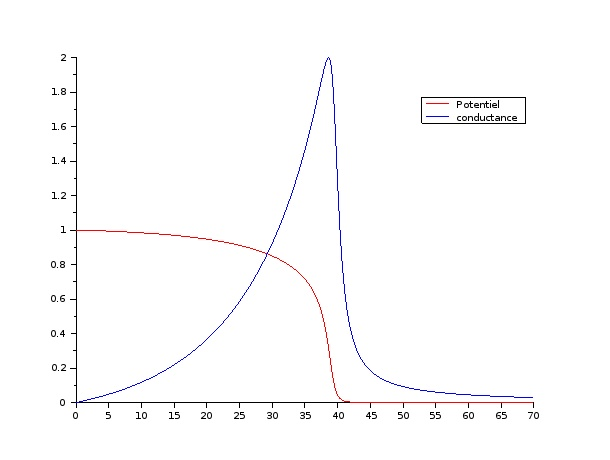
\includegraphics[width=8 cm]{Solution0D.jpeg}
		\caption{ Solution approchée du modéle 0D }
	\end{center}
	\end{figure}
	
\section{Simulation en dimension supérieure}
	\stepcounter{question_num}
	\paragraph{Question \arabic{question_num} \\}
	La fonction $gen\_grille$ permet de créer une grille $ \Omega $ où chaque point contient les valeurs de e et r demandées.


	\stepcounter{question_num}
	\paragraph{Question \arabic{question_num} \\}
	Cette fonction construit une matrice de taille $n^2*n^2$ comme définie dans le sujet. Pour cette fonction, nous avons choisi de construire les diagonales exterieurs puis de compléter la matrice en construisant les "blocs" $T_{k}$ séparément.
	
	\stepcounter{question_num}
	\paragraph{Question \arabic{question_num} \\}
	Cette fonction utilise la fonction précédente pour réduire la taille de la matrice creuse créée.
	
	\stepcounter{question_num}
	\paragraph{Question \arabic{question_num} \\}
	 Nous avons mesuré le temps d'execution d'une multiplication entre la matrice et un vecteur. Nous obtenons des résultats trés différents entre L et Ls :
	\begin{figure}[H]
	\begin{center}
		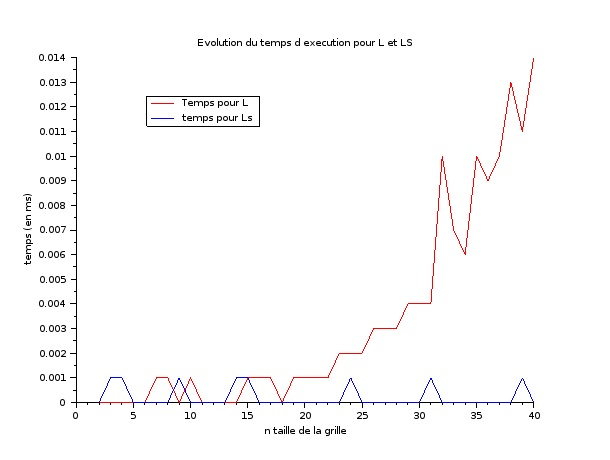
\includegraphics[width=8 cm]{Comparaison_L_Ls.jpeg}
		\caption{ Comparaison des temps d'exécutions de L et Ls}
	\end{center}
	\end{figure}
	
	Pour Ls, les calculs sont trés rapides (presque instantanés). Mais pour Ls, les calculs sont exponentiels. En effet, pour Ls, la taille augmente de façon linéaire alors que pour L la taille augmente en $n^{4}$.
	
	\stepcounter{question_num}
	\paragraph{Question \arabic{question_num} \\}
	Cette fonction prend en argument: la taille de la grille, le temps maximum, les grilles E et R initiale et une fonction. Ainsi cette fonction calcule les $45^{ere}$ grilles E et R (afin de ne pas surcharger la mémoire). Elle résout donc ce probléme approché pendant un petit nombre de pas.
	
	\stepcounter{question_num}
	\paragraph{Question \arabic{question_num} \\}
	Afin de vérifier la fonction précédente, nous allons la tester avec un systéme dont la solution est :
	%%u a (x, y, t) = cos(πx) cos(πy)e −t et v a = cos(2πx) cos(2πy)e −t
	\[
	\left\{
	\begin {array}{r c l}
	u_a(x,y,t)=& cos(\pi x)cos(\pi y)e^{-t}\\
	u_a(x,y,t)=& cos(2 \pi x)cos(2 \pi y)e^{-t}
	\end {array}
	\right.
	\]
	
	On obtient alors le sytéme suivant :
	\[
	\left\{
	\begin {array}{r c l}
	\frac{de}{dt} =& -e\\
	\frac{dr}{dt} =& -r
	\end {array}
	\right.
	\]
	
	Malheureusement, notre fonction ne semble pas fonctionnée correctement. Nous obtenons des résultats incohérents :
	\begin{figure}[H]
	\begin{center}
		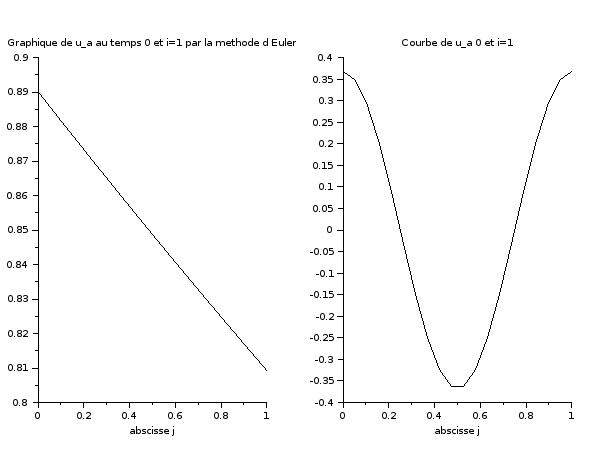
\includegraphics[width=8 cm]{question10.jpeg}
		\caption{ état de $u-{v}$ au temps 2*dt}
	\end{center}
	\end{figure}
	
	\stepcounter{question_num}
	\paragraph{Question \arabic{question_num} \\}
	Nous ne pouvons répondre à cette question sans la précedente. Voila néanmoins ce que nous obtenons :
	\begin{figure}[H]
	\begin{center}
		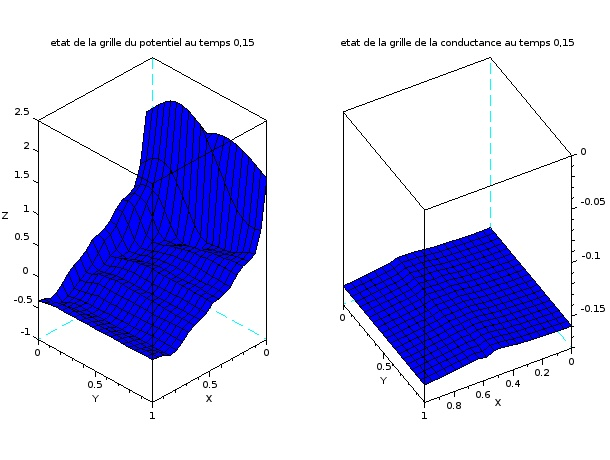
\includegraphics[width=8 cm]{question11.jpeg}
		\caption{}
	\end{center}
	\end{figure}

\section{Une méthode d’ordre supérieur }

		
			
\end{document}
